\documentclass{llncs}
\usepackage{makeidx}
\usepackage[english]{babel}
\usepackage[utf8]{inputenc}
\usepackage{amsmath}
\usepackage{url}
\usepackage{fancyvrb}
\usepackage[spanish]{babelbib}
\usepackage{graphicx}


%%%%%%%%%% Text with box
\usepackage{tikz}
\usetikzlibrary{shadows}

\newcommand{\raisedtext}[1]{
  \vspace{2mm}
  \begin{tikzpicture}
    [baseline=(X.base)]\node [drop shadow,fill=white,draw,very thin] (X) {#1};
  \end{tikzpicture}
  \vspace{2mm}
}
%%%%%%%%%%%%%%%%%%%



\graphicspath{ {img/} }

\urldef{\mails}\path|{fbarrios,fjlopez}@fi.uba.ar| 

\newtheorem{definicion}{Definition} 

\begin{document}

\frontmatter

\title{Variations of TextRank for Automated Summarization}
\titlerunning{Variantes de TextRank} 


\maketitle

\begin{abstract}
This article describes our proposal for new variants of the TextRank algorithm for automated summarization of texts. We describe the generalities of the TextRank algorithm on its original version and the different variations of the algorithm that we created. Some of these variants achieve a significative improvement over the original algorithm using the same metrics and dataset as the original publication. 
\keywords{TextRank variations, automated summarization, Information Retrieval ranking functions}

\end{abstract}

\section{Introduction}
We can describe the process of automated summarization as the extraction of the most important sentences in a document. Using different levels of compression a summarized version of the document of arbitrary length can be obtained. The TextRank algorithm is one of the most used methods for this task. TextRank builds a graph of sentences for a document and then applies PageRank to obtain a score for each sentence. In this article we describe several different proposals for the construction of the TextRank graph and report the results obtained with them.

The first section of this article describes previous work in the area and the TextRank algorithm in general. Then we report the results obtained for the different variations of the algorithm. Finally we describe the different metrics used for the evaluation of the results obtained from the proposed changes and the datasets used for these tests.

\section{Previous work}
The field of automated summarization has attracted interest since the late 50's \cite{luhn}. Traditional methods for text summarization analyze the frequency of words or sentences in the first paragraphs of the text to identify the most important lexical elements. Several statistical models have been developed based on training corpora to combine different heuristics using keywords, position and length of sentences, word frequency and titles \cite{hovy}. On a different approach, some algorithms analyze the semantic structure of the different textual units in a document with the goal of separating those that take a significative role in the representation of the document \cite{marcu}.

Other methods are based in the representation of the text as a graph: the most important sentences are the most connected ones in the graph and are used for building a final summary \cite{barzilay}. These algorithms use different information retrieval techniques to identify similar sentences and determine the most important ones \cite{salton}. The TextRank algorithm developed by Mihalcea and Tarau \cite{mihalcea-tarau} and the LexRank algorithm by Erkan and Radev \cite{erkan} are based in ranking the lexical units of the text (sentences or words).

\section{TextRank}

\subsection{Description}
TextRank is an unsupervised algorithm for the automated summarization of texts that can also be used to obtain the most important keywords in a document. It was introduced in 2004 by Rada Mihalcea and Paul Tarau in \cite{mihalcea-tarau}.

The algorithm applies a variation of PageRank \cite{pageetal98} over a graph constructed specifically for the task of summarization. This method provides an understanding of the structure of the document identifying its principal concepts without the need of previous training. Since the algorithm is based on PageRank it uses the idea of ranking of the elements in the graph, the most important elements are the ones that better describe the text. This approach allows TextRank to build summaries without the need of a training corpus or labeling and allows the use of the algorithm with different languages as long as there is a way to build the graph of sentences for it.

\subsection{Text as a Graph}
For the task of automated summarization, TextRank models any document as a graph using sentences as nodes \cite{introductionir}. A function to compute the similarity of sentences is needed to build edges in between. This function is used to weight the graph edges, the higher the similarity between sentences the more important the edge between them will be in the graph. In the domain of a Random Walker, as used frequently in PageRank, we can say that we are more likely to go from one sentence to another if those sentences are very similar. 

The similarity function can use several different ideas. It can be based on the semantic of the sentences, on their proximity in the text, common words, and many other different metrics. The goal of this article is to experiment with these functions and report the results obtained when used along with TextRank.

The function featured in the original algorithm can be formalized as:

\begin{definicion}
Given $S_i$, $S_j$ two sentences represented by a set of $n$ words that in 
$S_i$ are represented as $S_i = w_{1}^{i}, w_{2}^{i},..., w_{n}^{i}$. The similarity function for $S_i$, $S_j$ can be defined as:


\begin{equation}
Sim(S_{i},S_{j}) = \frac{ | \{   w_{k} | w_{k} \in S_{i} \& w_{k} \in S_{j}   \}  | }    
                              {  log(|S_{i}|) + log(|S_{j}|)  }
\end{equation}


\end{definicion}

The result of this process is a dense graph representing the document. From this graph, PageRank is used to compute the importance of each vertex. The most significative sentences are selected and presented in the same order as they appear in the document as the summary.


\section{Experiments}

\subsection{Our Variations}
This section will describe the different variations that we propose over the original TextRank algorithm. These ideas are based in changing the way in which distances between sentences are computed to weight the edges of the graph used for PageRank. We found some of these variations to produce significative improvements over the original algorithm.

\subsubsection{Longest Common Substring}
From two sentences we identify the longest common substring (LCS) and report the similarity to be its length.

\subsubsection{Cosine Distance}
The cosine similarity is a metric widely used to compare texts represented as vectors. We used a classical TF-IDF model to represent the documents as vectors and computed the cosine between vectors as a measure of similarity. Since the vectors are defined to be positive, the cosine results in values in the range [0,1] where a value of 1 represents identical vectors and 0 represents orthogonal vectors.

\subsubsection{BM25}
BM25 / Okapi-BM25 is a ranking function widely used as the state of the art for Information Retrieval tasks. BM25 is a variation of the TF-IDF model using a probabilistic model.

\begin{definicion}
Given two sentences R, S, BM25 is defined as:

\begin{equation}
BM25(R,S) = \sum_{i=1}^{n} IDF(s_i) \cdot \frac{f(s_i, R) \cdot (k_1 + 1)}{f(s_i, R) + k_1 \cdot (1 - b + b \cdot \frac{|R|}{avgDL})}
\end{equation}

where $k$ and $b$ are parameters. We used $k = 1.2$ and $b = 0.75$. $avgDL$ is the average length of the sentences in our collection.
\end{definicion}

This function definition implies that if a word appears in more than half the documents of the collection, it will have a negative value. Since this can cause problems in the next stage of the algorithm, we used the following correction formula:
                
\begin{equation}
 IDF(s_i) =
  \begin{cases}
       log(N - n(s_i) + 0.5) - log(n(s_i) + 0.5)    & \text{if }  n(s_i) > N/2\\
       \varepsilon \cdot avgIDF                     & \text{if }  n(s_i) \leq N/2\\
  \end{cases}
\end{equation}                
                
where $\varepsilon$ takes a value between 0.5 and 0.30 and $avgIDF$ is the average IDF for all terms.

We also used BM25+, a variation of BM25 that changes the way long documents are penalized.


\subsection{Evaluation}
For testing the proposed variations, we used the database of the 2002 Document Understanding Conference (DUC) \cite{duc2002-guidelines}. The corpus has 567 documents that are summarized to 20\% of their size, and is the same corpus used in \cite{mihalcea-tarau}. 

To evaluate results we used version 1.5.5 of the ROUGE package \cite{Lin2004a}. The configuration settings were the same as those in DUC, where ROUGE-1, ROUGE-2 and ROUGE-SU4 were used as metrics, using a confidence level of 95\% and applying stemming. The final result is an average of these three scores.

To check the correct behaviour of our test suite we implemented the reference method used in \cite{mihalcea-tarau}, which extracts the first sentences of each document. We found the resulting scores of the original algorithm to be identical to those reported in \cite{mihalcea-tarau}: a 2.3\% improvement over the baseline.


\subsection{Results}
We tested LCS, Cosine Sim, BM25 and BM25+ as different ways to weight the edges for the TextRank graph. 
The best results were obtained using BM25 and BM25+. We achieved an improvement of 2.92\% above the original TextRank result using BM25 and $\varepsilon$ = 0.25. The following chart shows the results obtained for the different variations we proposed.

\begin{table}
\caption{Evaluation results for the proposed TextRank variations.}
\begin{center}
\begin{tabular}{l*{5}{c}r}
\hline
\rule{0pt}{12pt}
Method & ROUGE-1 & ROUGE-2 & ROUGE-SU4 & Improvement \\[2pt]
\hline\rule{0pt}{12pt}\mbox{}\par\nobreak
BM25 (Neg to epsilon) & 0.4042 & 0.1831 & 0.2018 & 2.92\% \\
BM25+ (Neg to epsilon) & 0.404 & 0.1818 & 0.2008 & 2.60\% \\
Cosine TF-IDF & 0.4108 & 0.177 & 0.1984 & 2.54\% \\
BM25+ (IDF = log(N/NI)) & 0.4022 & 0.1805 & 0.1997 & 2.05\% \\ 
BM25 (IDF = log(N/NI)) & 0.4012 & 0.1808 & 0.1998 & 1.97\% \\ 
Longest Common Substring & 0.402 & 0.1783 & 0.1971 & 1.40\% \\
BM25+ (Neg to zero) & 0.3992 & 0.1803 & 0.1976 & 1.36\% \\ 
BM25 (Neg to zero) & 0.3991 & 0.1778 & 0.1966 & 0.89\% \\
\textbf{TextRank} & \textbf{0.3983} & \textbf{0.1762} & \textbf{0.1948} & \textbf{--}\\
BM25 & 0.3916 & 0.1725 & 0.1906 & -1.57\% \\
BM25+ & 0.3903 & 0.1711 & 0.1894 & -2.07\% \\
DUC Baseline & 0.39 & 0.1689 & 0.186 & -2.84\% \\ [2pt]
\hline
\end{tabular}
\end{center}
\end{table}

\begin{figure}[h!]
    \centering
    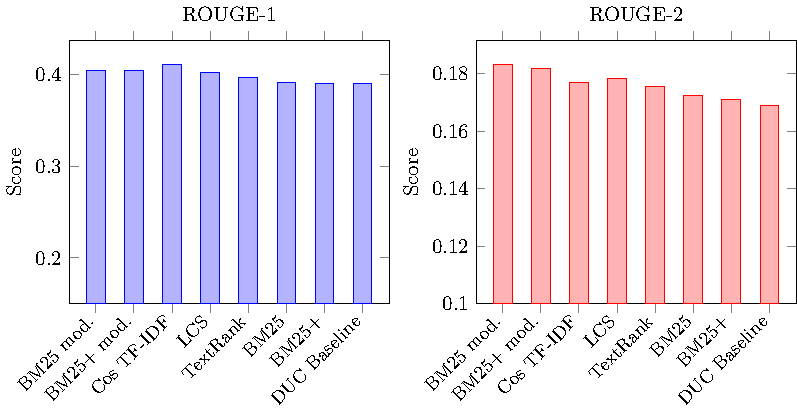
\includegraphics[width=1\textwidth]{rouge-scores-en.pdf}
    \caption{ROUGE-1 and ROUGE-2 scores comparison.}
\end{figure}

The result of Cosine Similarity was also satisfactory with a 2.54\% improvement over the original method. The LCS variation also improved the original TextRank algorithm with 1.40\% total improvement.

The performance in time was also improved. We could process the 567 documents from the DUC2002 database in 84\% of the time needed in the original version.


\section{Example}
A sample document from the 2002 DUC (Document Understanding Conference) dataset \cite{duc2002-guidelines} is shown in Figure \ref{fig:text}. The modified TextRank algorithm builds the graph shown in Figure \ref{fig:graph} and produces the summary shown in Figure \ref{fig:bm25}. The summary generated by the original method is shown in Figure \ref{fig:textrank}.

\begin{figure}
\caption{Sample document from the DUC 2002 corpus.}
\label{fig:text}
\raisedtext{{\scriptsize \parbox{\linewidth}{
\begin{enumerate}
\item Super Bowl Was Lowest-Rated in 21 Years
\item By RONALD BLUM AP Sports Writer NEW YORK (AP)
\item The San Francisco 49ers' 55-10 rout of the Denver Broncos was the lowest-rated Super Bowl in 21 years and the third-lowest ever.
\item The game on CBS averaged a 39.0 rating and a 63 share, the lowest Super Bowl rating since 1969, when the New York Jets' 16-7 victory over Baltimore got a 36.0 on NBC for the worst rating ever, A.C. Nielsen Co. said today.
\item The rating is a percentage of the nation's televisions; each point represents 921,000 homes.
\item The share is the percentage of the televisions on at the time.
\item Despite the low rating, Sunday's game was seen by about 108.5 million people, making it the ninth most-watched TV show ever in the United States behind eight Super Bowls and the final episode of ``MASH''.
\item The higher viewership was made possible by the annual increase in the number of homes with television.
\item ``Given the expected blowout, the numbers are completely understandable and we're happy to have a 39,'' said Susan Kerr, director of programming for CBS Sports.
\item ``It's still a remarkable rating for prime time''.
\item The 49ers won by the biggest margin in Super Bowl history.
\item Only the 1969 and 1968 Super Bowls had lower ratings; Green Bay's 33-14 victory over Oakland in 1968 got a 36.8.
\item The first Super Bowl was in 1967.
\item The highest-rated Super Bowl was in 1982, when the 49ers' 26-21 victory over Cincinnati got a 49.1 on CBS.
\item Last year's San Francisco-Cincinnati Super Bowl, won by the 49ers 20-16, got a 43.5 rating and was seen in 39.3 million homes, according to Nielsen estimates.
\item This year's game was seen in about 35.9 million homes.
\item Viewership of the 5 p.m. game this year peaked at a 41.6 rating and a 69 share from 6 p.m. to 6:30 p.m., dropping off as it became clear that Denver would not rally.
\item The pregame show got a 39.0 rating and a 63 share and the postgame show got a 22.5 rating and a 35 share.
\item The musical ``Annie,'' which was on ABC opposite the game, got a 9.4 rating.
\item ``Life Goes On'' on NBC got a 6.0 rating and ``Love With a Twist'' on NBC a 7.6 . 
\end{enumerate}
}}}
\end{figure}

\begin{figure}[h!]
    \centering
    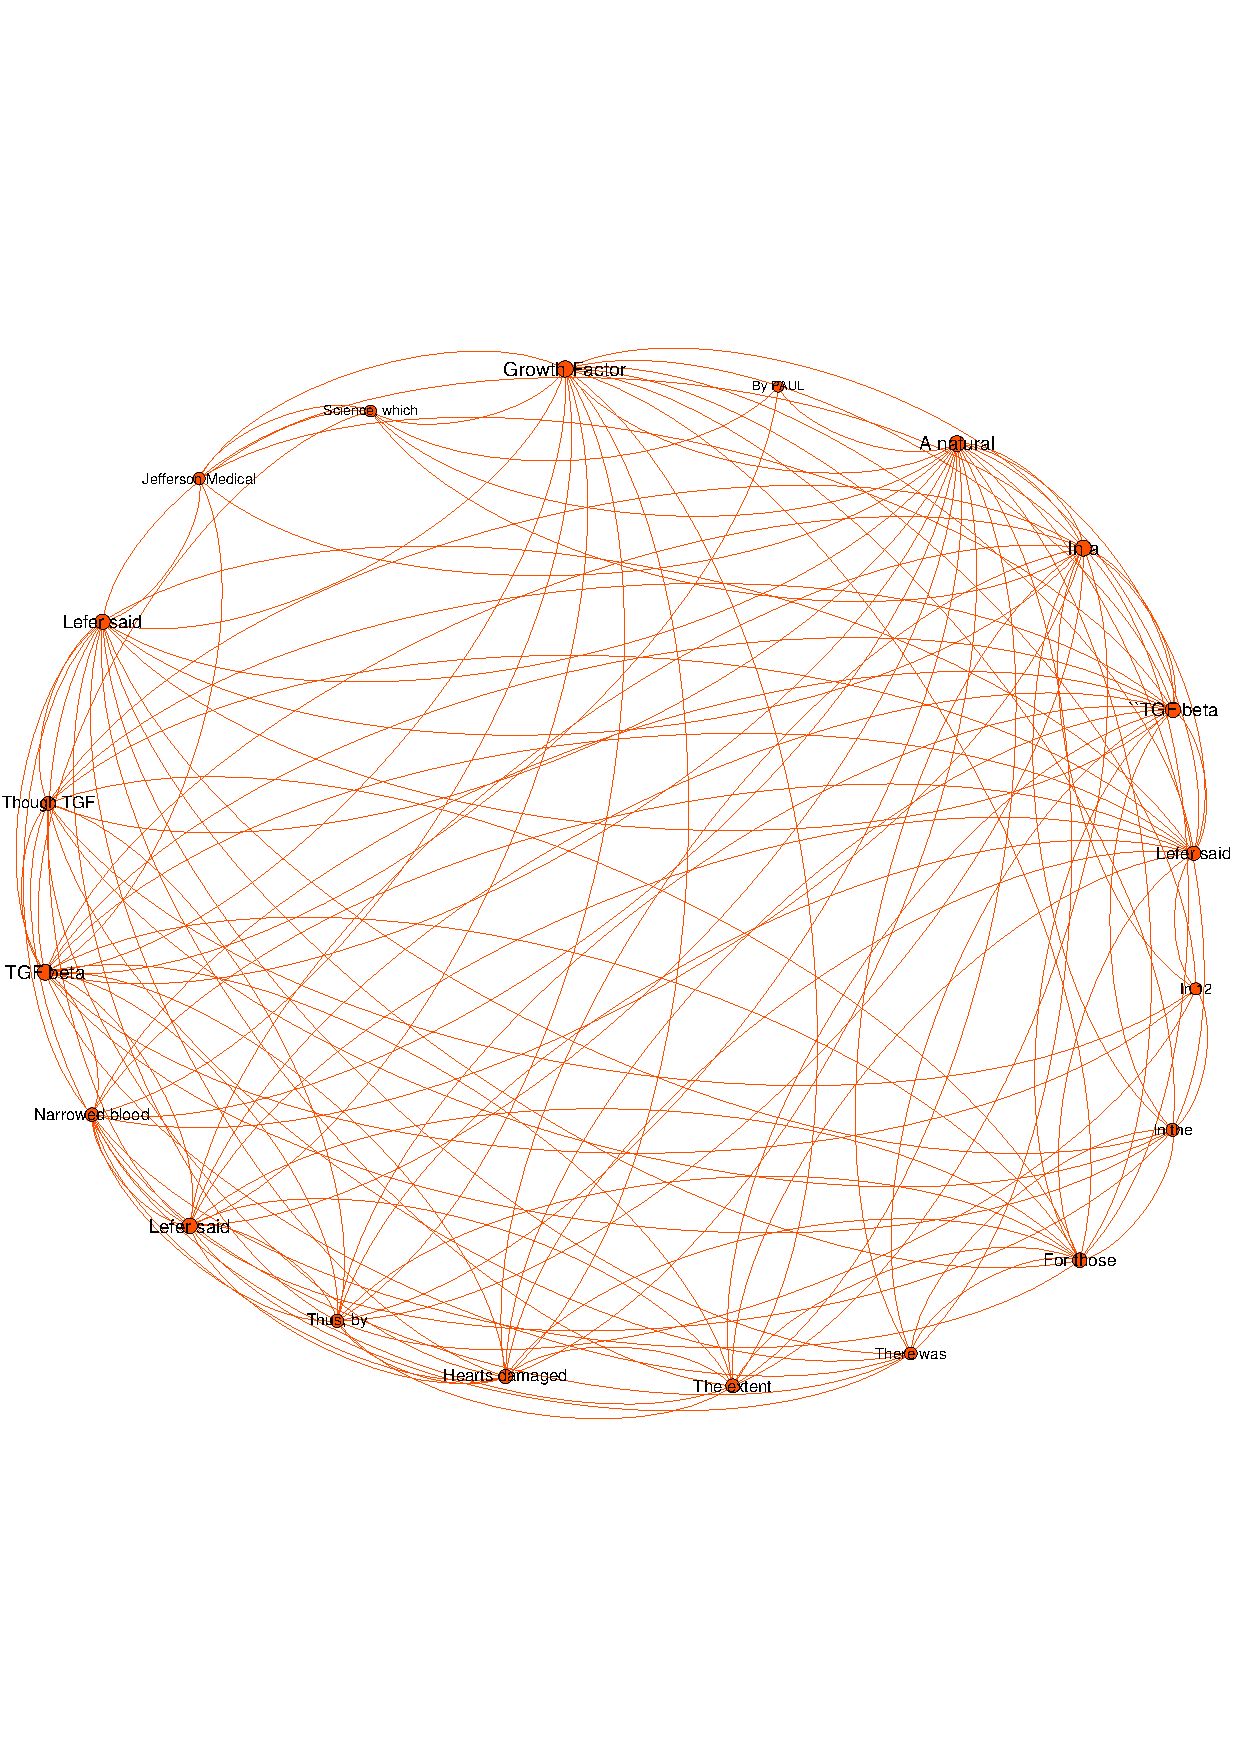
\includegraphics[trim = 0mm 50mm 0mm 50mm, clip, scale=0.15,width=1\textwidth]{graph.pdf}
    \caption{Graph created from the sample text.}
    \label{fig:graph}
\end{figure}

\begin{figure}
\caption{Summary generated by modified TextRank with BM25.}
\label{fig:bm25}
\raisedtext{{\scriptsize \parbox{\linewidth}{The San Francisco 49ers' 55-10 rout of the Denver Broncos was the lowest-rated Super Bowl in 21 years and the third-lowest ever.
The game on CBS averaged a 39.0 rating and a 63 share, the lowest Super Bowl rating since 1969, when the New York Jets' 16-7 victory over Baltimore got a 36.0 on NBC for the worst rating ever, A.C. Nielsen Co. said today.
The highest-rated Super Bowl was in 1982, when the 49ers' 26-21 victory over Cincinnati got a 49.1 on CBS.
Last year's San Francisco-Cincinnati Super Bowl, won by the 49ers 20-16, got a 43.5 rating and was seen in 39.3 million homes, according to Nielsen estimates.}}}
\end{figure}


\begin{figure}
\caption{Summary generated by original TextRank from the sample text.}
\label{fig:textrank}
\raisedtext{{\scriptsize \parbox{\linewidth}{Super Bowl Was Lowest-Rated in 21 Years
The game on CBS averaged a 39.0 rating and a 63 share, the lowest Super Bowl rating since 1969, when the New York Jets' 16-7 victory over Baltimore got a 36.0 on NBC for the worst rating ever, A.C. Nielsen Co. said today.
The highest-rated Super Bowl was in 1982, when the 49ers' 26-21 victory over Cincinnati got a 49.1 on CBS.
Last year's San Francisco-Cincinnati Super Bowl, won by the 49ers 20-16, got a 43.5 rating and was seen in 39.3 million homes, according to Nielsen estimates.}}}
\end{figure}

\section{Reference Implementations and Gensim Contribution}
A reference implementation of our proposals was coded as a Python module. It can be obtained for testing and to reproduce results from an URL that will be provided in the non-anonymous version.

We also contributed the BM25-TextRank algorithm to the Gensim project \cite{rehurek_lrec}.

\section{Conclusions}
This work presented three different variations to the TextRank algorithm for automatic summarization. The three variations presented improved significantly the results of the algorithm using the same metric and database used in the original paper. Given that TextRank performs 2.84\% over the baseline, our improvement of 2.92\% over the TextRank result is an important result. 

The combination of TextRank with modern Information Retrieval ranking functions such as BM25 and BM25+ results in the creation of a robust method for automatic summarization that performs better than the standard techniques used previously. 

Based on this results we suggest the use of BM25 along with TextRank for the task of unsupervised automatic summarization of texts. The results obtained and the examples analyzed show that this variation is better than the original TextRank algorithm without a performance penalty.

\bibliography{report-en}{}
\bibliographystyle{splncs03}


\end{document}
